\section{Introduction}
\label{sec:intro}

\kwa{(Paragraph removed.)}

GPU memory capacity has become a bottleneck for the continued growth of LLMs.
As Figure~\ref{fig:trend_scale} shows, the increase of GPU memory capacity is around 60\% slower than the LLM size scaling speed and the GPU FP16 throughput improvement. About 80\% of the GPU memory used to train recent LLMs consists of activations~\cite{liuWinnerTakeAllColumnRow2023,korthikantiReducingActivationRecomputation2022}, the intermediate tensors produced by forward propagation and reused in backward propagation.
Furthermore, the memory needed for activations is growing more rapidly than any other memory use, making GPU memory a more severe constraint for future LLM training (see Section~\ref{sec:llm_scaling} for details).


Common mitigations are to reduce batch size or through gradient accumulation.  With gradient accumulation, a batch is divided into micro-batches that are processed separately between gradient updates.  Although gradient accumulation has been adopted by many LLMs~\cite{jiangMegaScaleScalingLarge2024,shoeybiMegatronLMTrainingMultiBillion2020a,workshopBLOOM176BParameterOpenAccess2023}, the GPU computation stack is not designed for small inputs, and both mitigations lead to device under-utilization~\cite{DissectingBatchingEffects,anthonyCaseCoDesigningModel2024} and suboptimal math library performance~\cite{aminabadiDeepSpeedInferenceEnabling2022}. 
Intuitively, a smaller batch size might reduce total training computation through faster convergence. However, LLM trainers have identified a critical batch size for each model, below which convergence speed increases negligibly or even decreases~\cite{kaplanScalingLawsNeural2020,mccandlishEmpiricalModelLargeBatch2018}.  Notably, critical batch size grows during training as training loss is reduced.

Another common approach to reducing GPU memory use is activation checkpointing.  With this strategy, only some activations are kept in GPU memory, while others are flushed and then recomputed during backward propagation.  For a model with $L$~layers, activation checkpointing can reduce memory requirements from $O(L)$ to $O(\sqrt{L})$~\cite{chenTrainingDeepNets2016}.  However, as we show in Section~\ref{sec:llm_scaling}, even this reduction is insufficient to eliminate the bottleneck posed by the GPU memory limits for future LLMs.



\begin{figure}[!t]
\centering
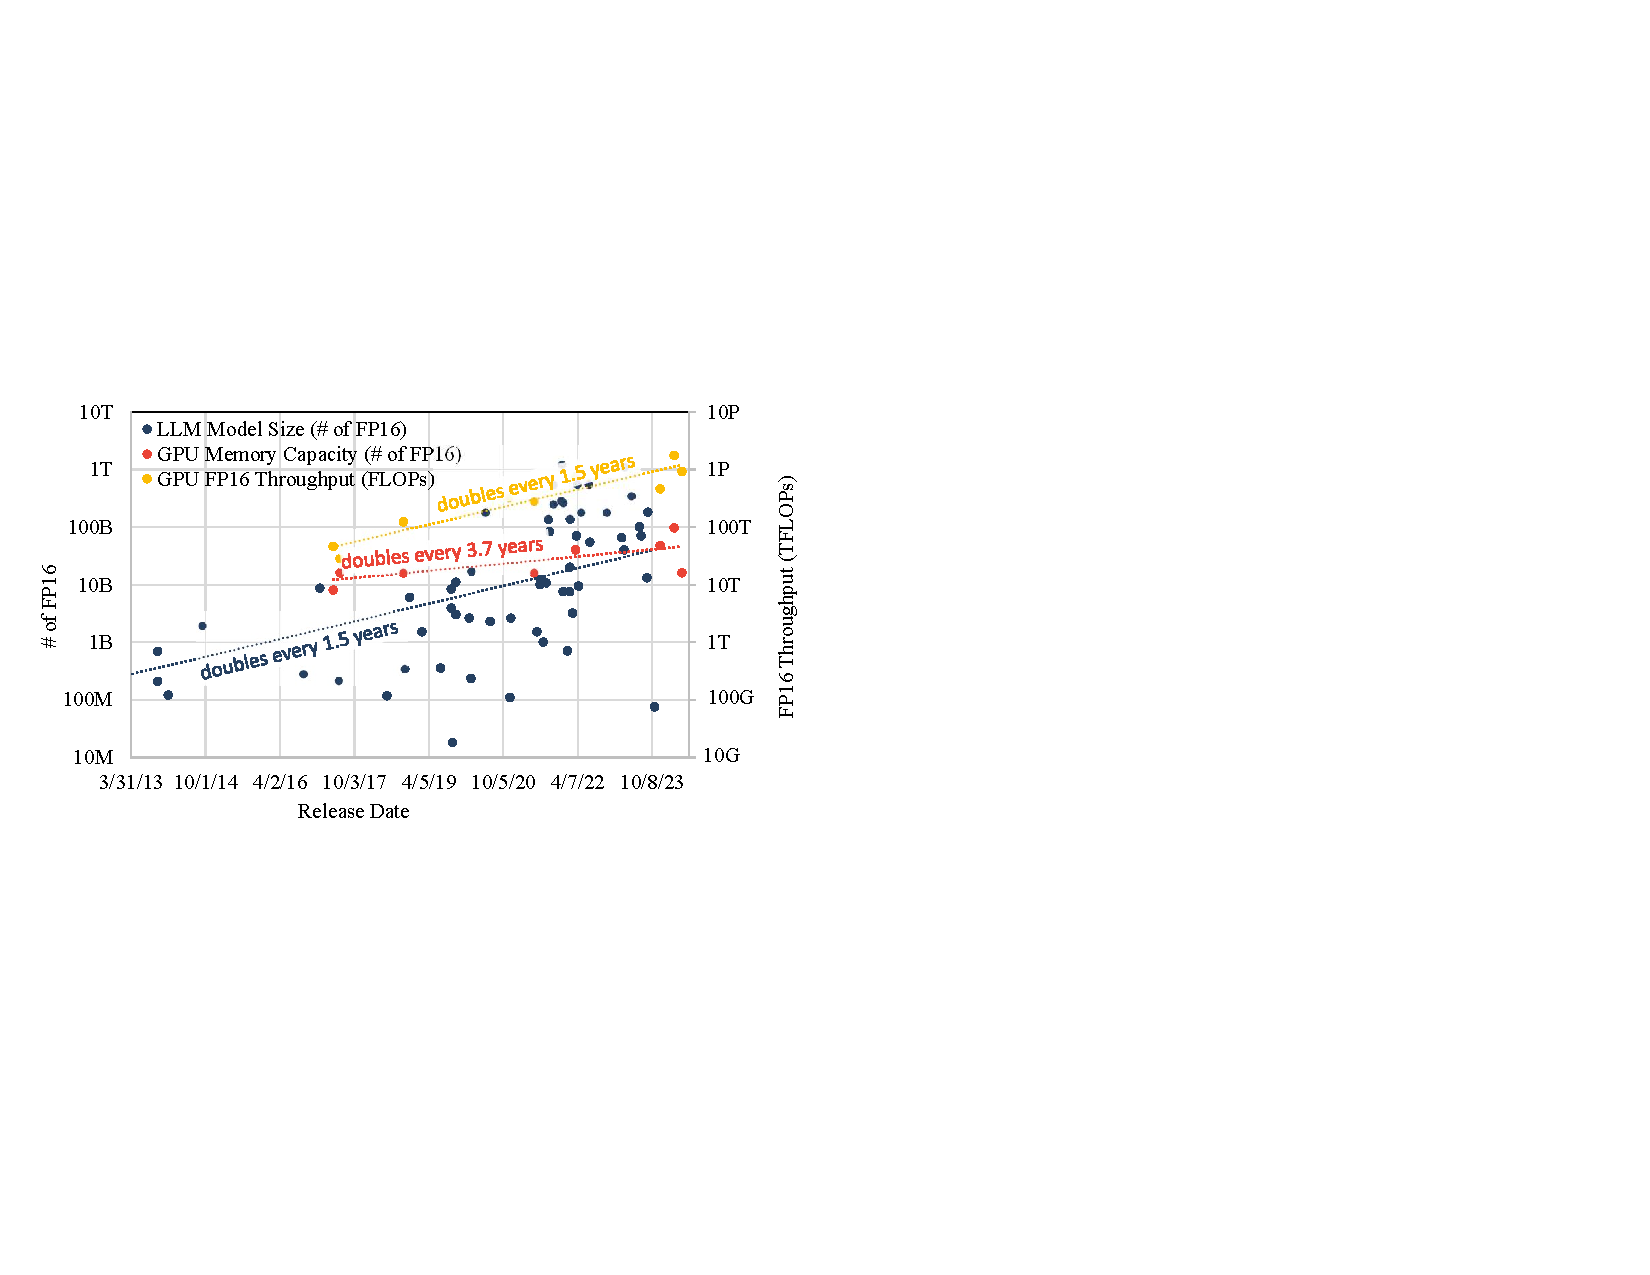
\includegraphics[width=\linewidth]{figures/SSDTrain/trend_scale_aux_words.pdf}
\caption{\label{fig:trend_scale} The growth of FP16 throughput (right vertical axis) of GPUs for deep learning training is aligned with the model size of LLMs (left vertical axis), but GPU memory capacity (left vertical axis) falls behind~\cite{theepochaiAnnouncingEpochAI2023}. The horizontal axis shows the release date.  Points represent both Nvidia 100-level GPUs since K100 and Google TPUs. The growth rate of FP16 throughput (yellow dotted line) is more than 2$\times$ of that of the memory capacity growth rate (red dotted line).}
\end{figure}

This chapter proposes SSDTrain, a software framework that offloads activations to NVMe SSDs and reloads activations just before they are needed in backward propagation.  SSDTrain can fully overlap activation transfers with computation, reducing activation memory usage without incurring significant performance overhead. 

SSDs are a more attractive target than main~(CPU) memory for several reasons. First, as illustrated in Figure~\ref{fig:current_sys}, clusters and cloud instances~\cite{microsoftNDA100V4series2024,googleGPUMachineTypes,ncsaDeltaProjectProfile} typically have limited host memory capacity (100--250 GB per GPU), while SSDs offer much greater capacity. Host memory capacity is further consumed by input data, checkpointing buffers, and other training management buffers, leaving even less capacity for activation offloading. \kwc{In contrast, as modeled in Section~\ref{sec:projected_life}, the activation size per GPU per training step in large LLM models can reach hundreds of GBs or even TBs, exceeding the capacity of host memory. Additionally, as Section~\ref{sec:llm_scaling} will detail, SSD capacity is increasing faster than the main memory, making SSD the more viable choice in the future.} Second, host memory bandwidth is shared across training management tasks and offloaded computation~\cite{kamahoriFiddlerCPUGPUOrchestration2024,renZeROOffloadDemocratizingBillionScale2021,songPowerInferFastLarge2023} running on the host CPU~\kwc{(Please see further elaboration on \textbf{Swapping and offloading} in Section~\ref{sec:ssdtrain_related})}. \kwc{This shared usage can make host memory bandwidth both limited and unpredictable}~\cite{baeFlashNeuronSSDEnabledLargeBatch2021} for saving and restoring activations. In contrast, the SSD bandwidth can be dedicated to activation offloading during training. 
Third, SSDs are more elastic, both by adding more SSDs and even PCIe switches if necessary---as well as through the use of optional remote high-throughput storage~\cite{googleGoogleCloudHyperdisk,lockwoodArchitecturePerformancePerlmutter2024}. Such elasticity allows the data centers to keep up with the fast-growing size of activations. In contrast, the memory capacity of GPU cloud instances and cluster nodes is much more challenging to extend. 


SSDTrain makes the following main contributions:
\begin{enumerate}[1.]
\item To address the GPU memory capacity issue and the resulting GPU under-utilization during LLM model training, we design and implement the SSDTrain framework to offload activations in LLM training to NVMe SSDs. We demonstrate the viability of SSDTrain on large-scale systems by modeling the performance, estimated SSD lifespan, and the required per-GPU PCIe bandwidth. 
\item With all code in Python except for a tiny CUDA memory allocation API hooking library, SSDTrain works with the latest PyTorch and distributed frameworks, including Megatron~\cite{shoeybiMegatronLMTrainingMultiBillion2020a} and DeepSpeed~\cite{rasleyDeepSpeedSystemOptimizations2020}. We developed and tested SSDTrain with Megatron-DeepSpeed~\cite{microsoftMicrosoftMegatronDeepSpeedOngoing2019} on a two-GPU node with seven Intel Optane SSDs. 
\item Because SSDTrain overlaps the data transfer entirely with computation, it incurs almost no performance overhead. To achieve this, we introduce several optimization techniques, including tensor deduplication, tensor forwarding, and adaptive offloading algorithm. 
\item Evaluation shows SSDTrain achieves almost the same training time per step as the original system without SSDTrain while reducing the activations peak memory use by up to 47\%. We introduce the recompute-offload-keep (ROK) curve to compare the SSDTrain offloading with two other tensor placement strategies, keeping activations in memory and layerwise full recomputation. SSDTrain has the same performance as keeping activations in memory and a lower memory peak than activation checkpointing. 
\item \kwc{We further analyze how the reduced activation memory use may be leveraged to increase throughput by increasing micro-batch size and reducing pipeline parallelism bubbles.}
\end{enumerate}
